
\title{Lab Report 07 - Structure from Motion}
\author{
        Manuel Galliker  14-921-969 \\
                manuelga@student.ethz.ch
}
\date{\today}

\documentclass[12pt]{article}
\usepackage{graphicx}
\usepackage{float}
\begin{document}
\maketitle


\section{1. Feature extraction and initialization with epipolar geometry }

For the first part of the exercise the functions vl shift and vl ubcmatch were used to extract features and match them. 
The matching can be seen in the picture below:

\vspace{5mm}
\begin{figure}[H]
	\centering
	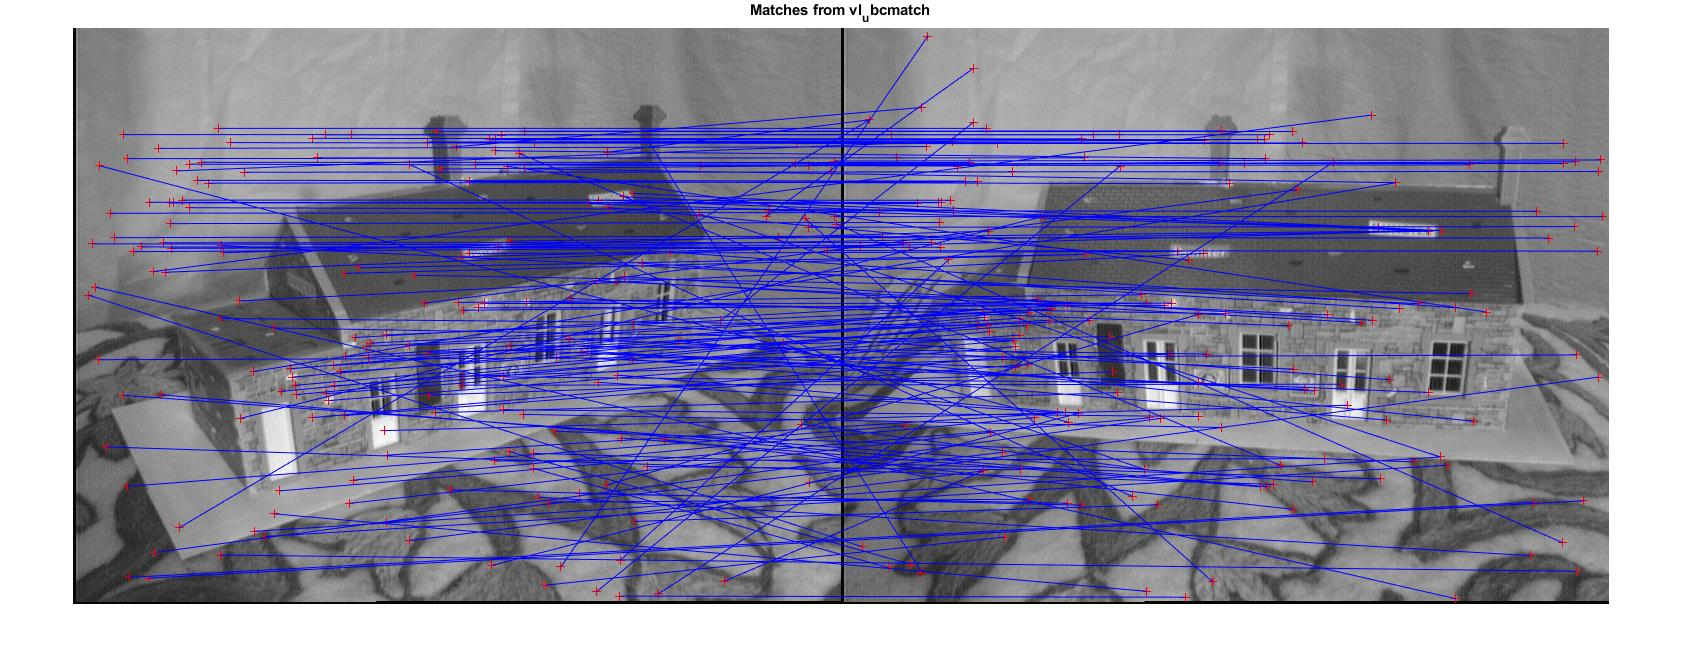
\includegraphics[width=1.1\textwidth]{1.jpg}
	\caption{matched features from vl ubcmatch}
	\label{fig1}
\end{figure}
\vspace{5mm}

As can be seen the set contains many correct matches but still a significant number of false positives. To improve this an 8-Point RANSAC Algorithm was used to compute a set of inliers. 


\vspace{5mm}
\begin{figure}[H]
	\centering
	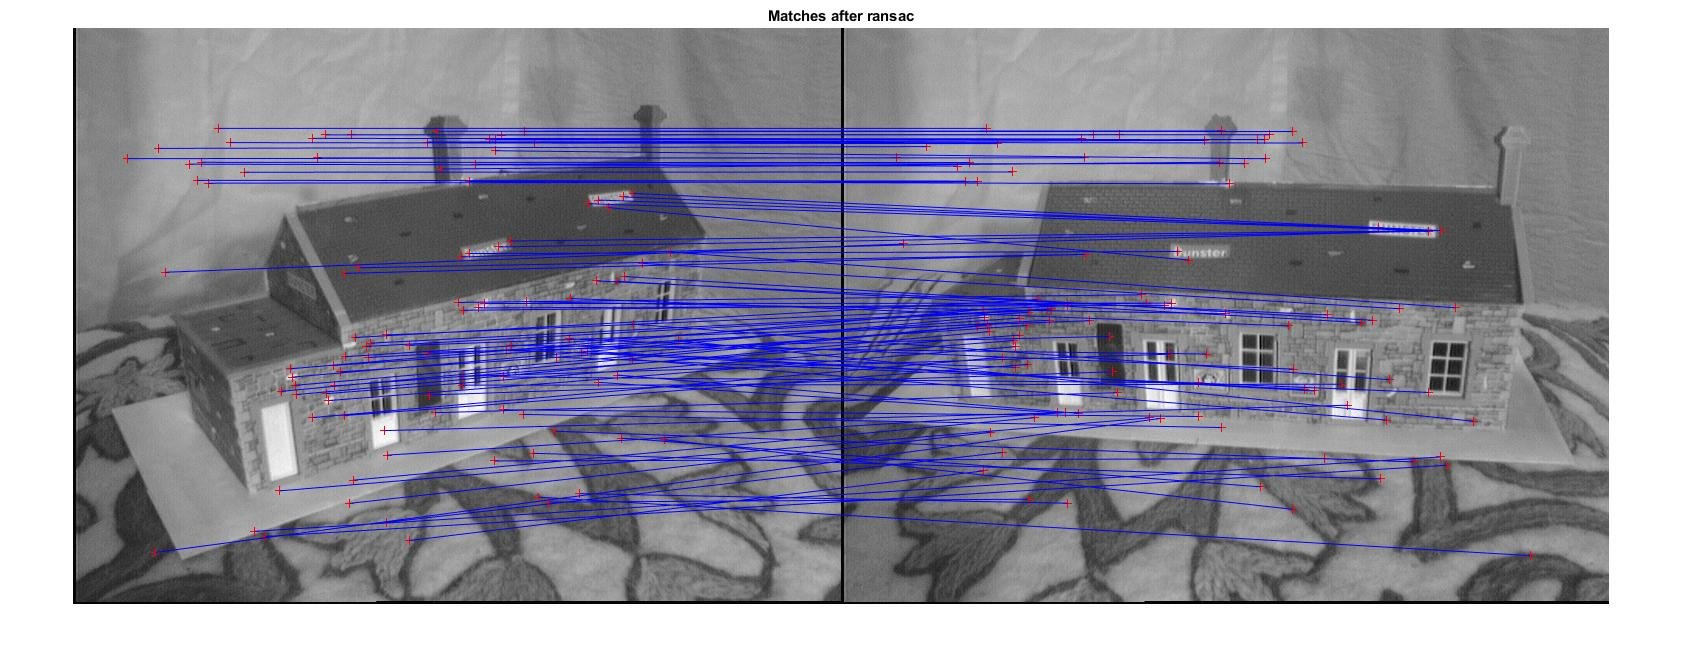
\includegraphics[width=1.1\textwidth]{2.jpg}
	\caption{Inlier matches after using 8-point RANSAC}
	\label{fig1}
\end{figure}
\vspace{5mm}



From these inliers the Fundamental Matrix F was computed which was then used, together with the intrinsic camera parameters K to calculate the Projection Matrix P. The projection Matrix Pand the calibrated corresponding points of the two images was then used in the provided $linearTriangulation$ function to compute the 3D Points.  
\newline
Last for this exercise the epipolar geometry of the corresponding images 0 and 4 are shown. As can be seen in the image the epipoles don't lie within the images.
\vspace{5mm}
\begin{figure}[H]
	\centering
	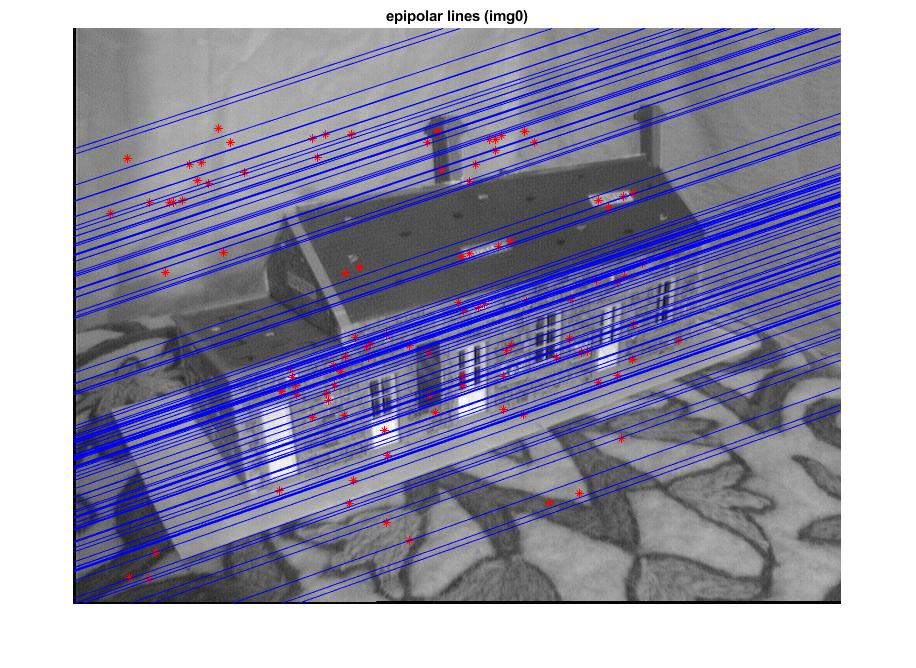
\includegraphics[width=1.1\textwidth]{ep0.jpg}
	\caption{Epipolar Lines in image 0}
	\label{fig1}
\end{figure}
\vspace{5mm}
\vspace{5mm}
\begin{figure}[H]
	\centering
	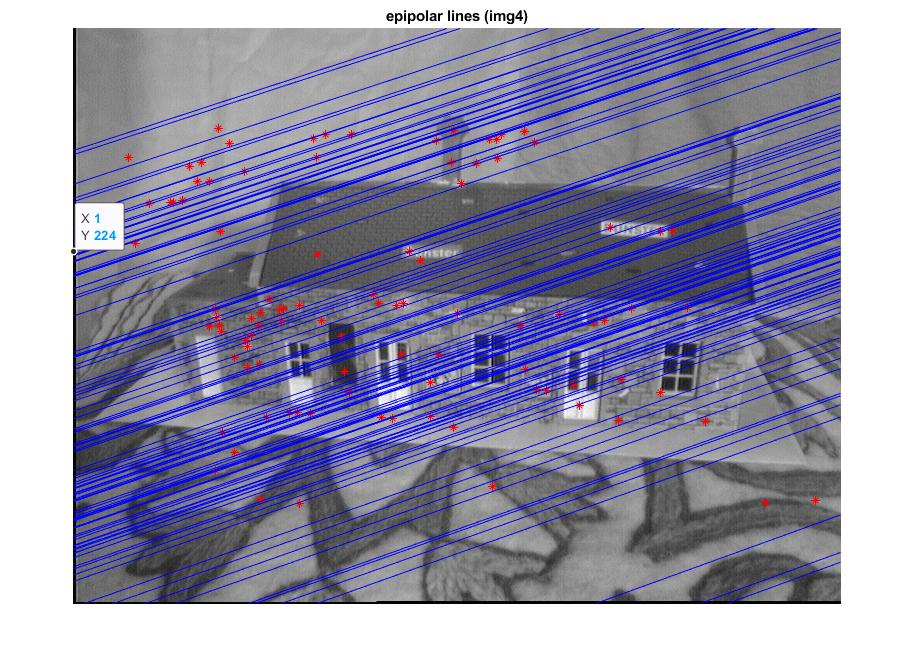
\includegraphics[width=1.1\textwidth]{ep4.jpg}
	\caption{Epipolar Lines in image 4}
	\label{fig1}
\end{figure}
\vspace{5mm}


\section{Additional Views}

As described in the Exercise two additional views were implemented. Hereby, $vl ubcmatch$ is calculated using the inlier descripters obtained in task 1 from image one and the descriptors from the new additional image. This insures that only points already present in the two most extreme views can be matched. Then the process is similar to the above with the exeption of a 6-point Ransac algorithm beeing used. 

\vspace{5mm}
\begin{figure}[H]
	\centering
	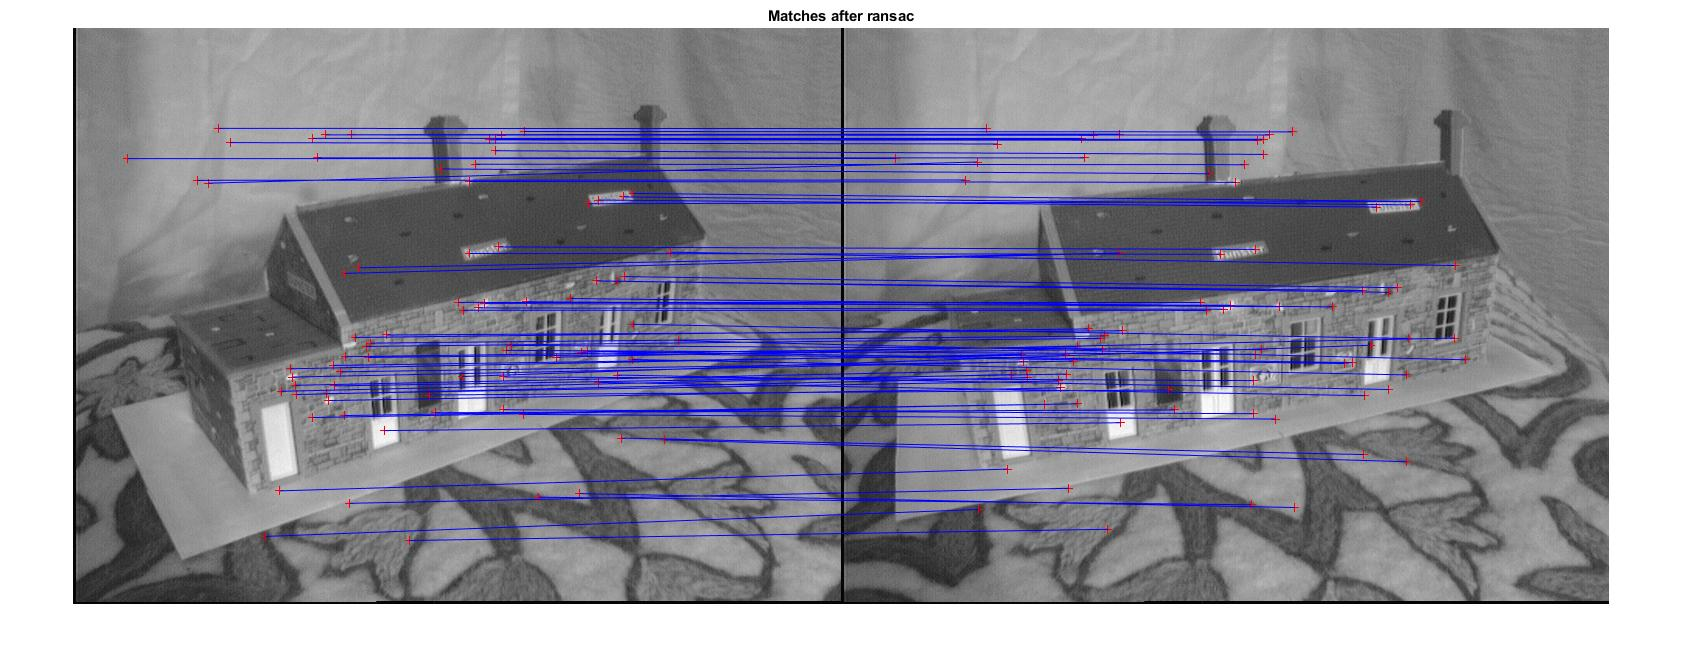
\includegraphics[width=1.1\textwidth]{3.jpg}
	\caption{Inlier matches between image 0 and 1 after using 6-point RANSAC}
	\label{fig1}
\end{figure}
\vspace{5mm}
\begin{figure}[H]
	\centering
	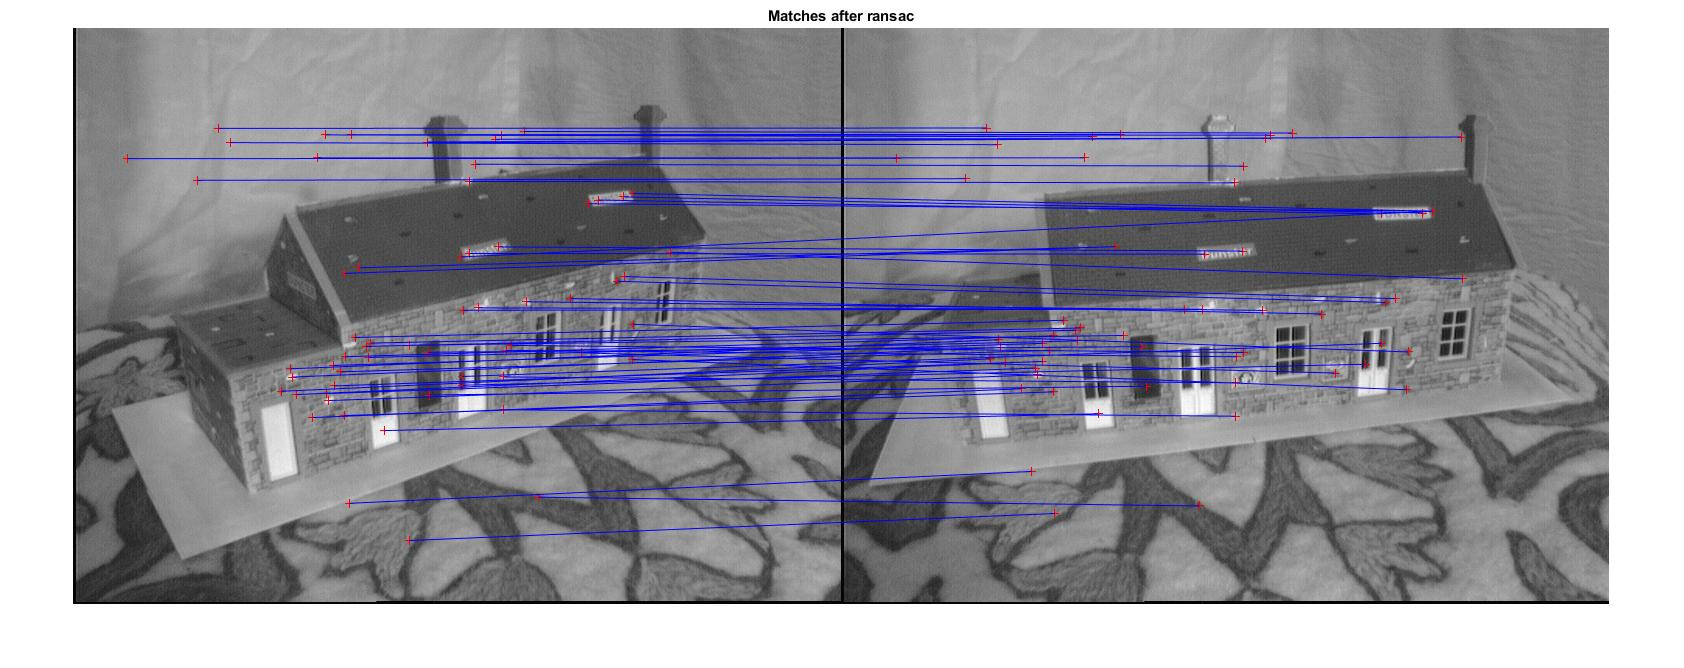
\includegraphics[width=1.1\textwidth]{4.jpg}
	\caption{Inlier matches between image 0 and 2 after using 6-point RANSAC}
	\label{fig1}
\end{figure}
\vspace{5mm}


\section{3D Plotting}

To plot all the points projected into 3D space the function plot3 was used with the 3 corresponding coordinates of the points. 

\vspace{5mm}
\begin{figure}[H]
	\centering
	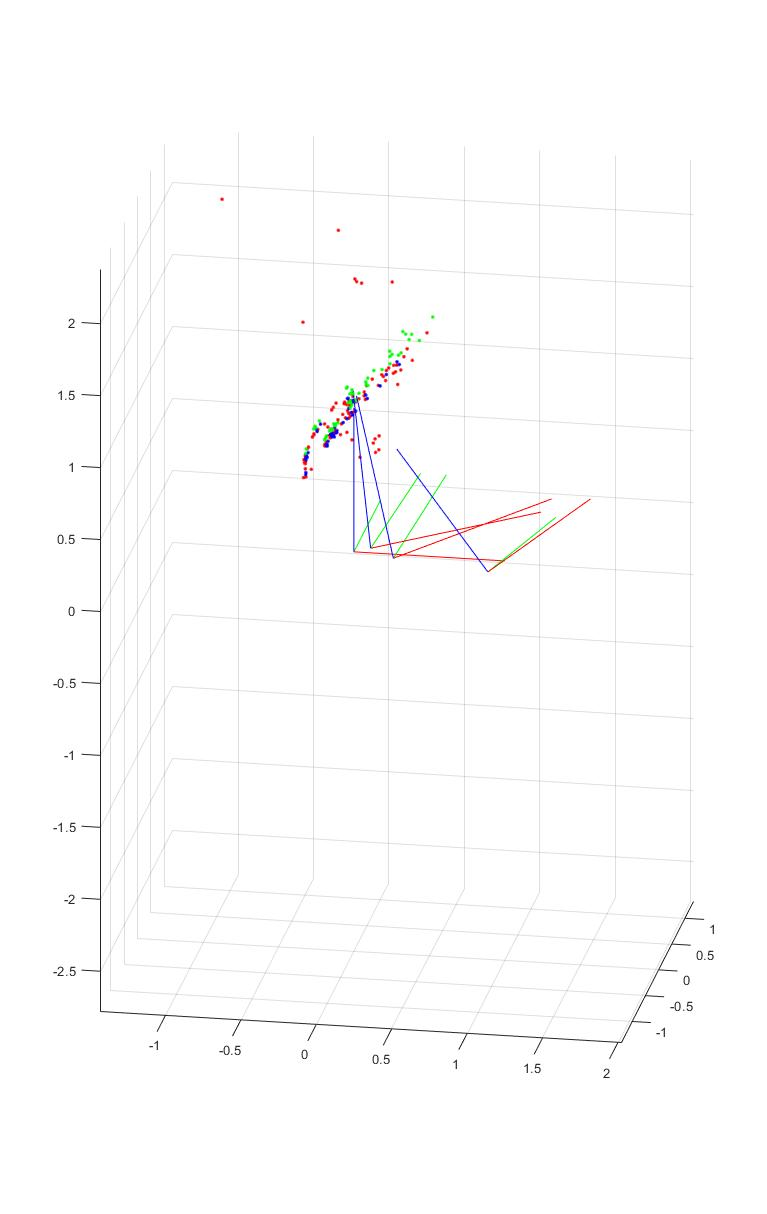
\includegraphics[width=0.8\textwidth]{5.jpg}
	\caption{3D view of the camera positions (img 0,1,2,4) and the reprojected 3D points for the three named image pairs}
	\label{fig1}
\end{figure}
\vspace{5mm}
\begin{figure}[H]
	\centering
	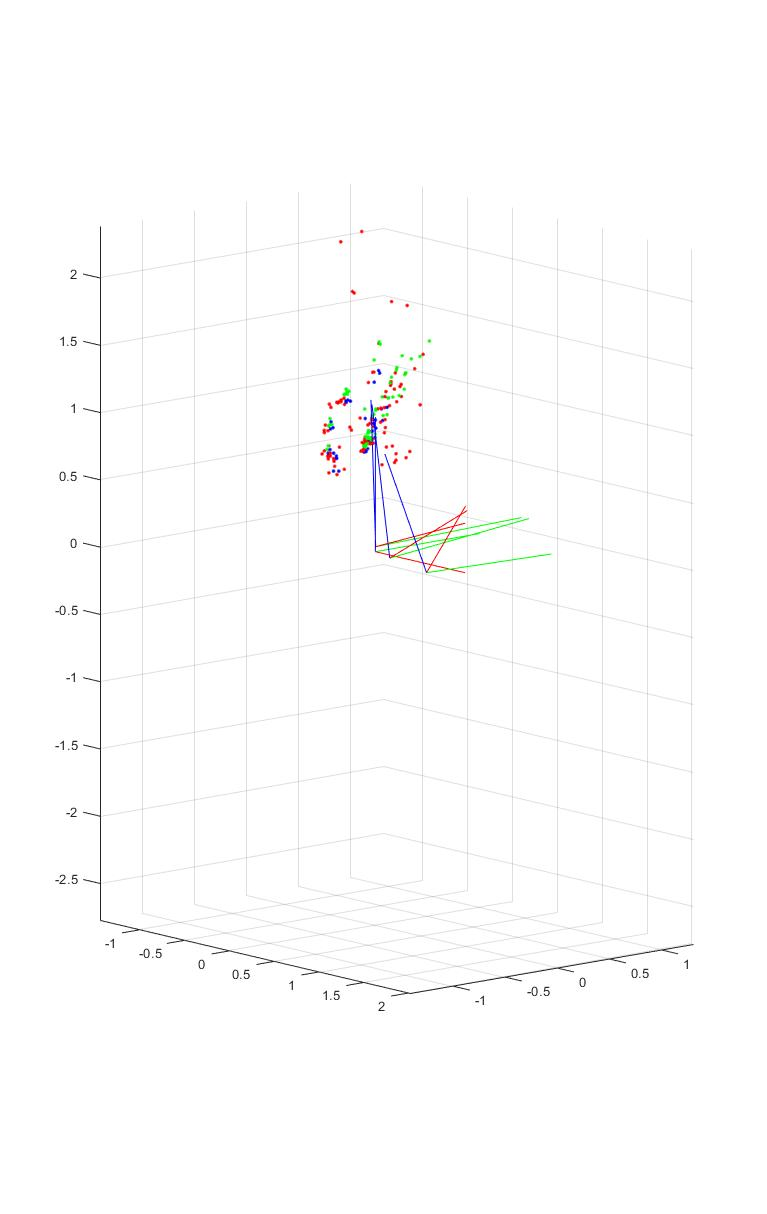
\includegraphics[width=0.8\textwidth]{6.jpg}
	\caption{3D view of the camera positions (img 0,1,2,4) and the reprojected 3D points for the three named image pairs}
	\label{fig1}
\end{figure}
\vspace{5mm}
\begin{figure}[H]
	\centering
	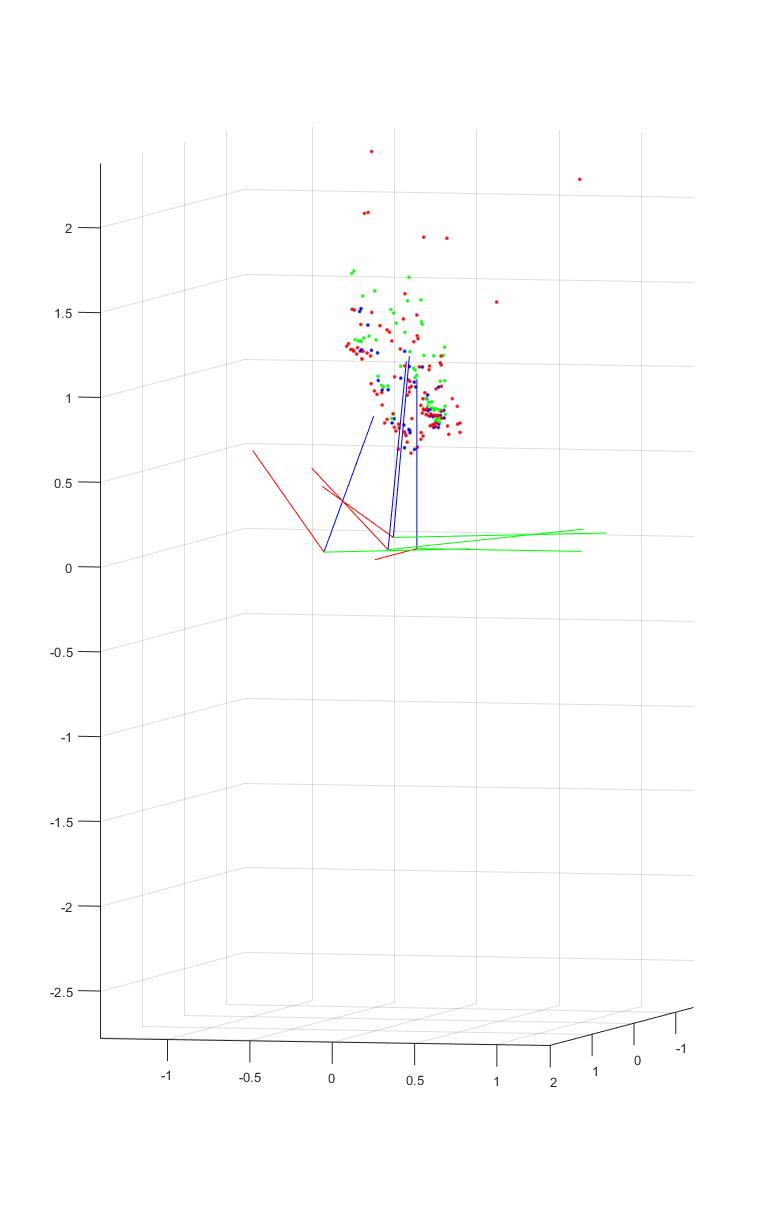
\includegraphics[width=0.8\textwidth]{7.jpg}
	\caption{3D view of the camera positions (img 0,1,2,4) and the reprojected 3D points for the three named image pairs}
	\label{fig1}
\end{figure}
\vspace{5mm}




\end{document}